% !TEX root = perelman-geometry.tex
%!TEX TS-program = pdflatex
%!TEX encoding = UTF-8 Unicode



\setchapterpreamble[o]{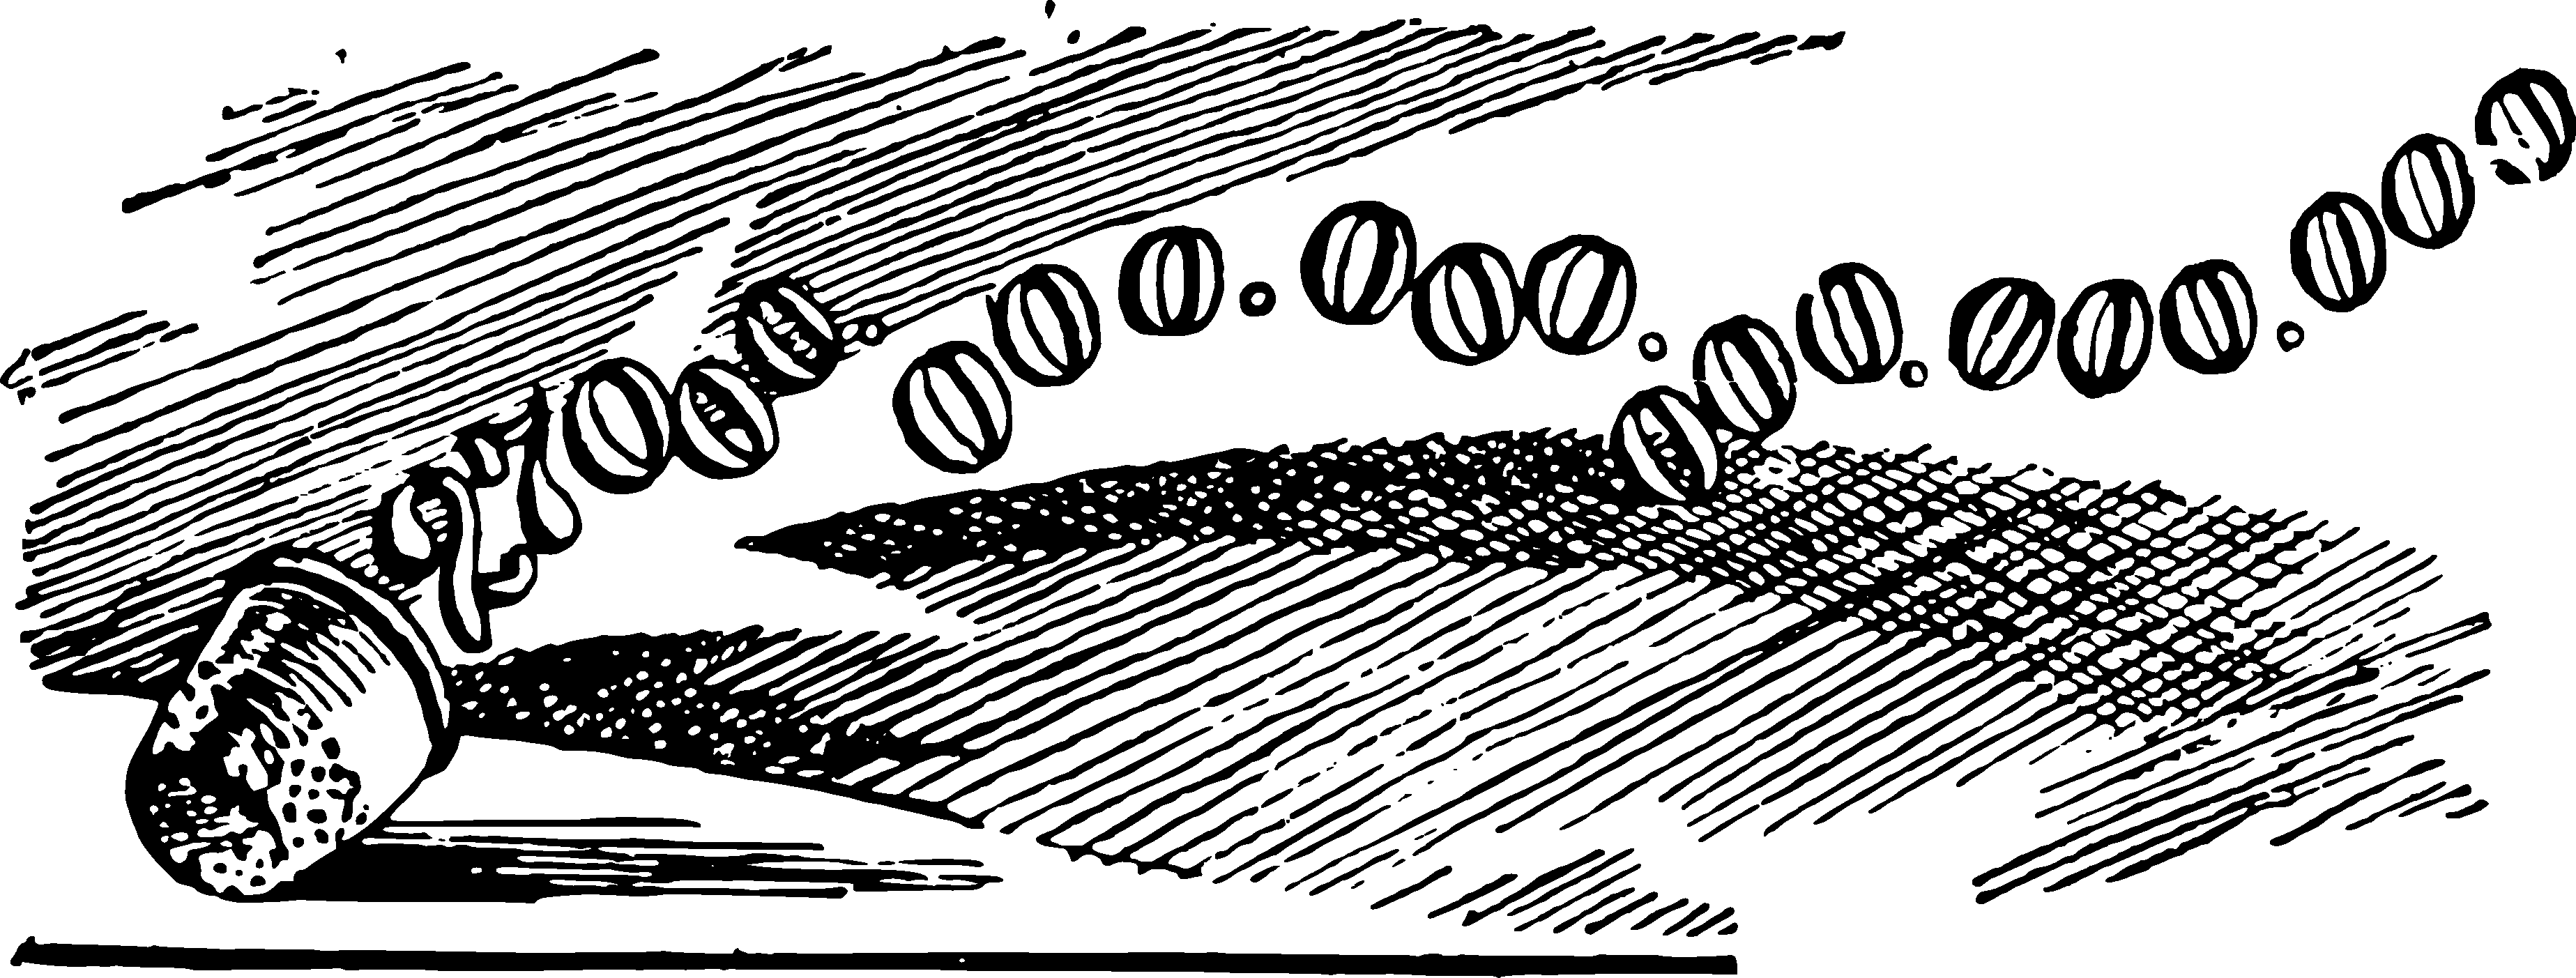
\includegraphics[width=1.2\textwidth]{figures/ch-11/fig-ch-11-head.pdf}\bigskip}

\chapter{Big And Small In Geometry}
\label{ch-11}



\section{In a Thimble}\marginnote{\large \num{21000000000000000000}}
\label{sec-11.1}

The number twenty-seven with eighteen zeros, written in the margin, can be read in different ways. Some will say: this is 27 trillion; others, for example financial workers, will read it as 27 quintillion, and still others will write it shorter: \num{27d18} and read it as 27 multiplied by ten to the eighteenth power.

But what can fit in such an incredible quantity in one thimble?

We are talking about particles of the air surrounding us. Like all substances in the world, air consists of molecules. Physicists have established that in every cubic centimetre (i.e., approximately in a thimble) of the air surrounding us at a temperature of \SI{0}{\degreeCelsius}, there are 27 trillion molecules. This is a numerical giant. To imagine it in any meaningful way is beyond the ability of even the liveliest imagination. Indeed, what can be compared to such a multitude? To the number of people in the world? But there are ``only'' two billion people on the globe (\num{2d9}), which is thirteen thousand million times smaller than the number of molecules in a thimble. 

Even if all the stars in the universe, visible to the most powerful telescope, were surrounded by planets like our Sun, and if each of these planets were inhabited as our Earth is, then even the number of inhabitants would not equal the molecular population of one thimble! If you attempted to count this invisible population, counting continuously, for example, at a rate of a hundred molecules per minute, it would take you at least five hundred billion years to count.

\begin{figure}[h!]
\centering
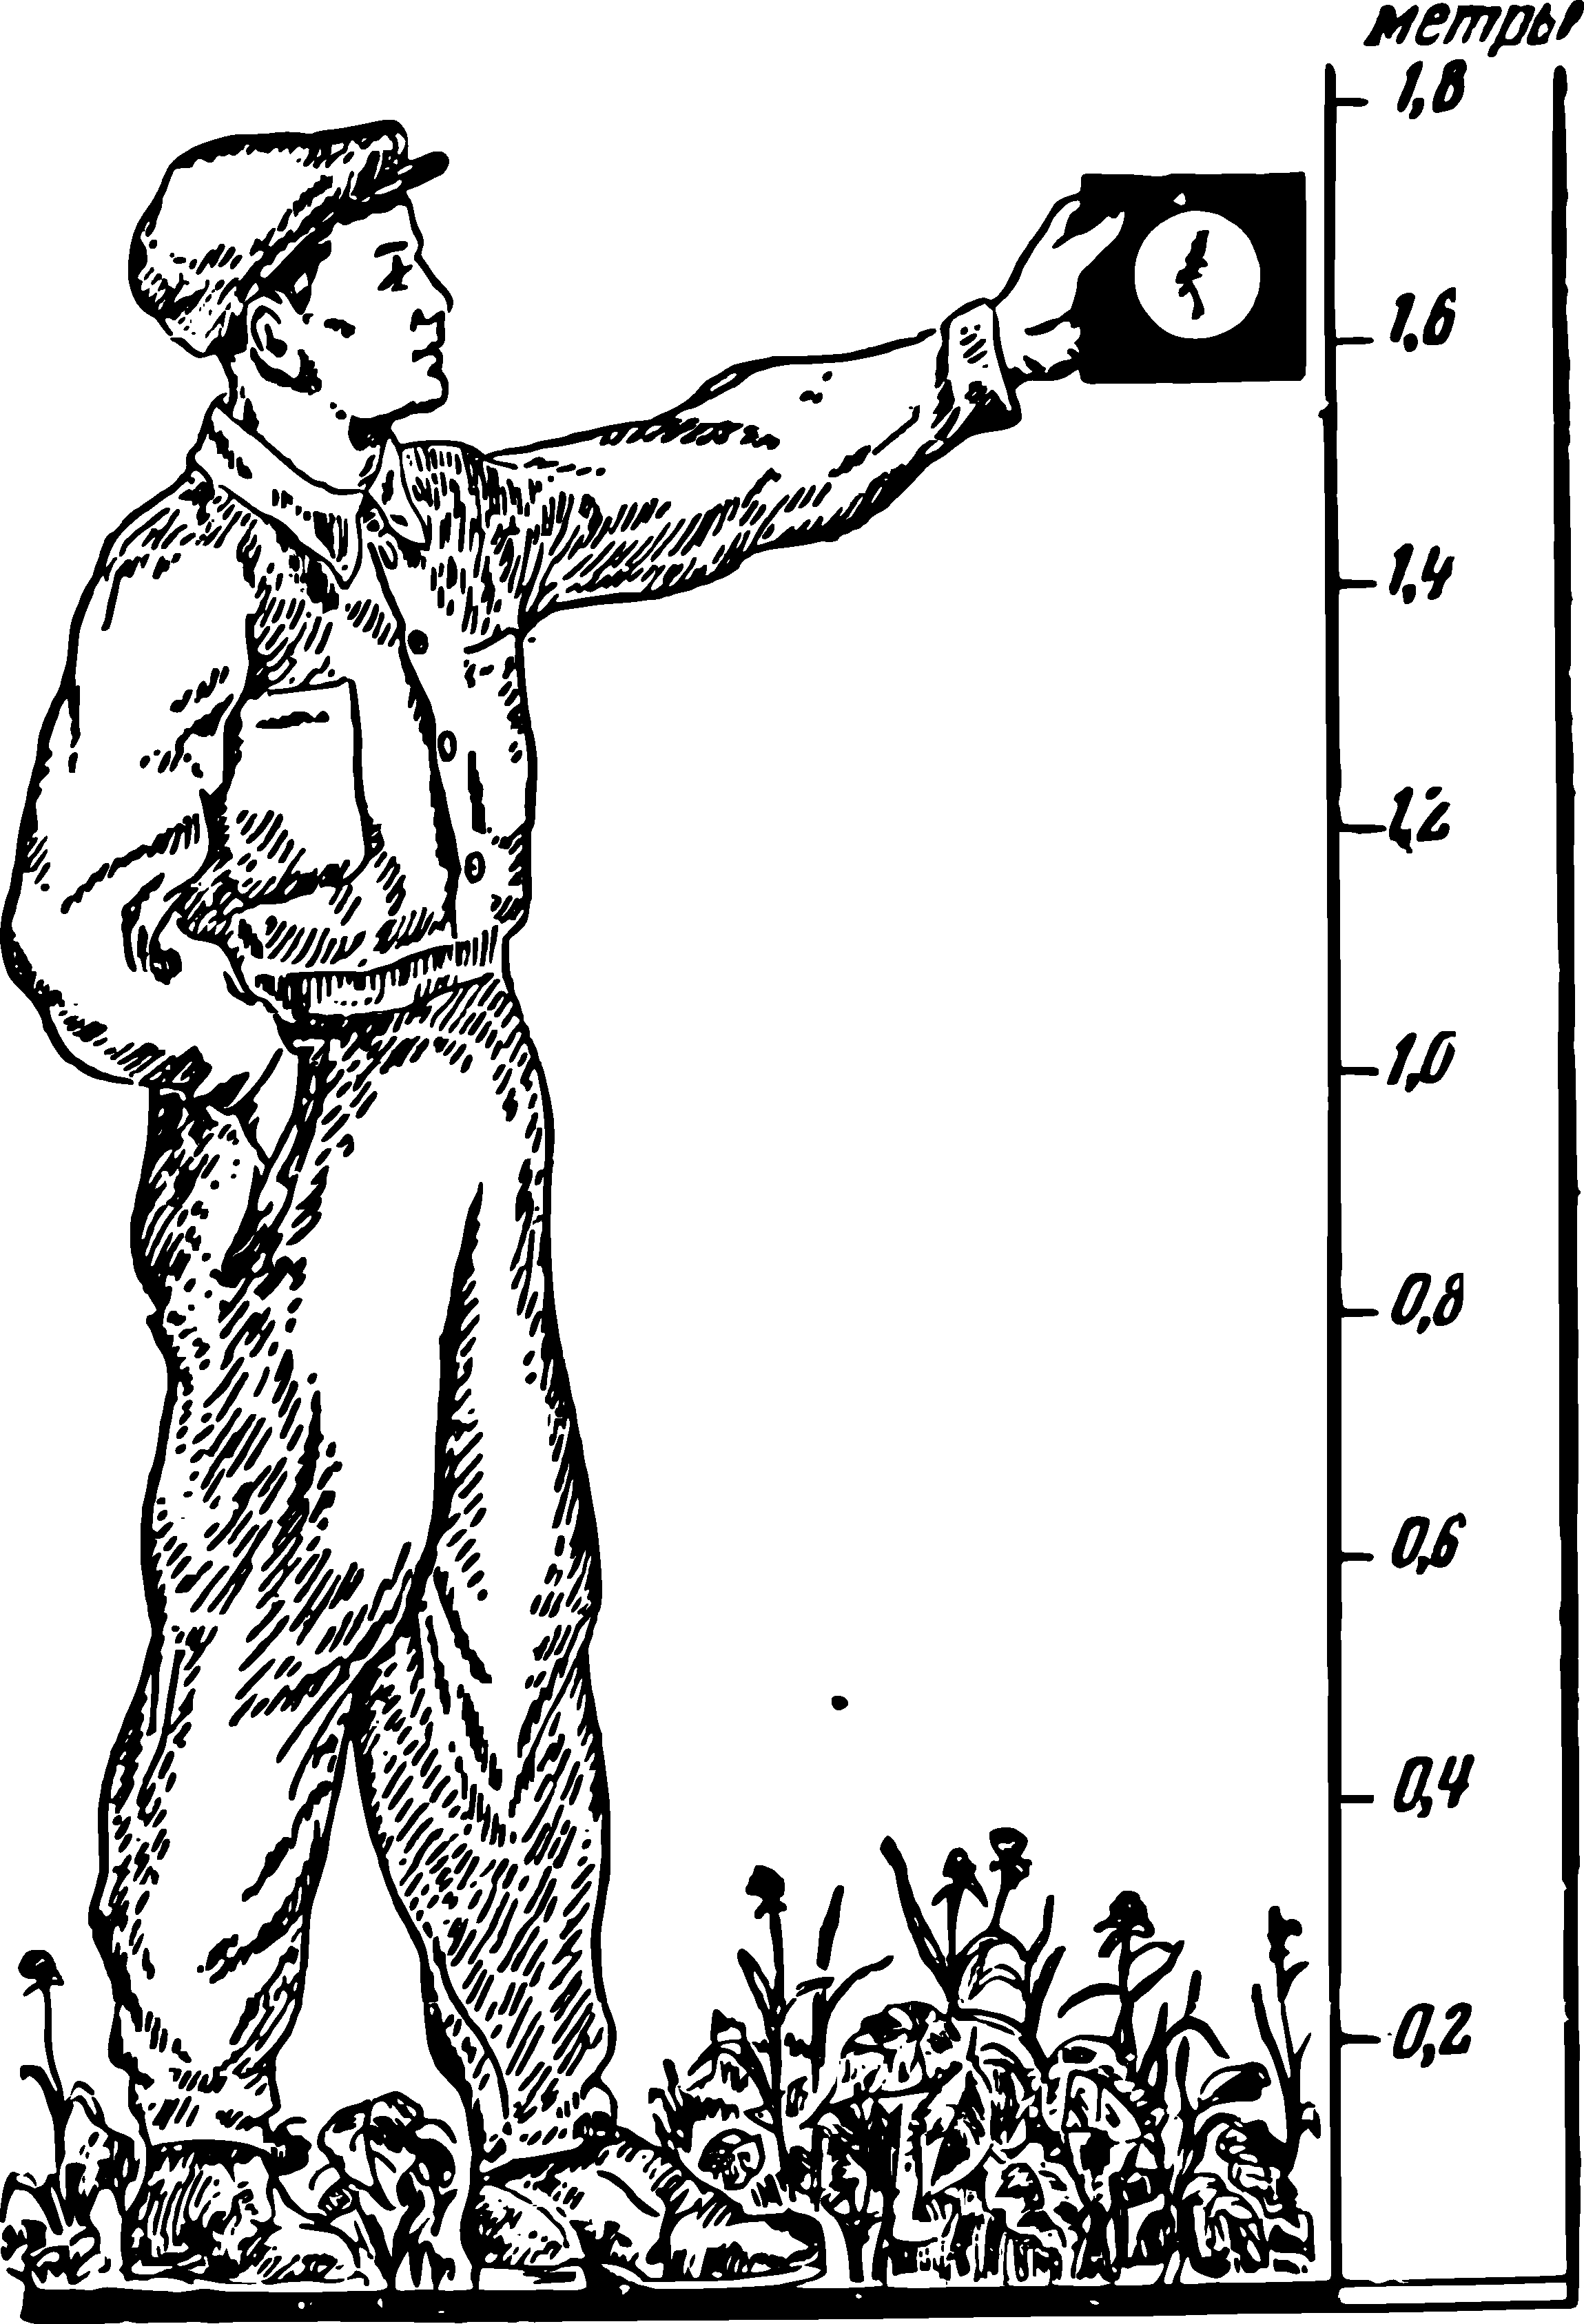
\includegraphics[width=0.6\textwidth]{figures/ch-11/fig-160.pdf}
\sidecaption{The young man looks at the typhus bacillus, magnified 1000 times.\label{fig-160}}
\end{figure}

Not everyone can clearly imagine even more modest numbers.

What do you envision when you are told, for example, about a microscope that magnifies by 1000 times? Not such a large number, just a thousand, but nevertheless, a thousandfold magnification is not perceived by everyone as it should be. We often fail to appreciate the true smallness of the objects we see under a microscope at such magnification. A typhoid bacterium, magnified by 1000 times, seems to us the size of a fly (see \figr{fig-160}) viewed at a distance of clear vision, i.e., \SI{25}{\centi\meter}. 


But how small is this bacterium really? Imagine that along with the magnification of the bacterium, you also magnified yourself by 1000 times. This means that your height would reach 1700 m! Your head would be above the clouds, and any of the new skyscrapers being built in Moscow would seem much lower than your knees (see \figr{fig-160}). The bacterium is as much smaller than the tiny fly as you are smaller than this imaginary giant.

\begin{figure}[h!]
\centering
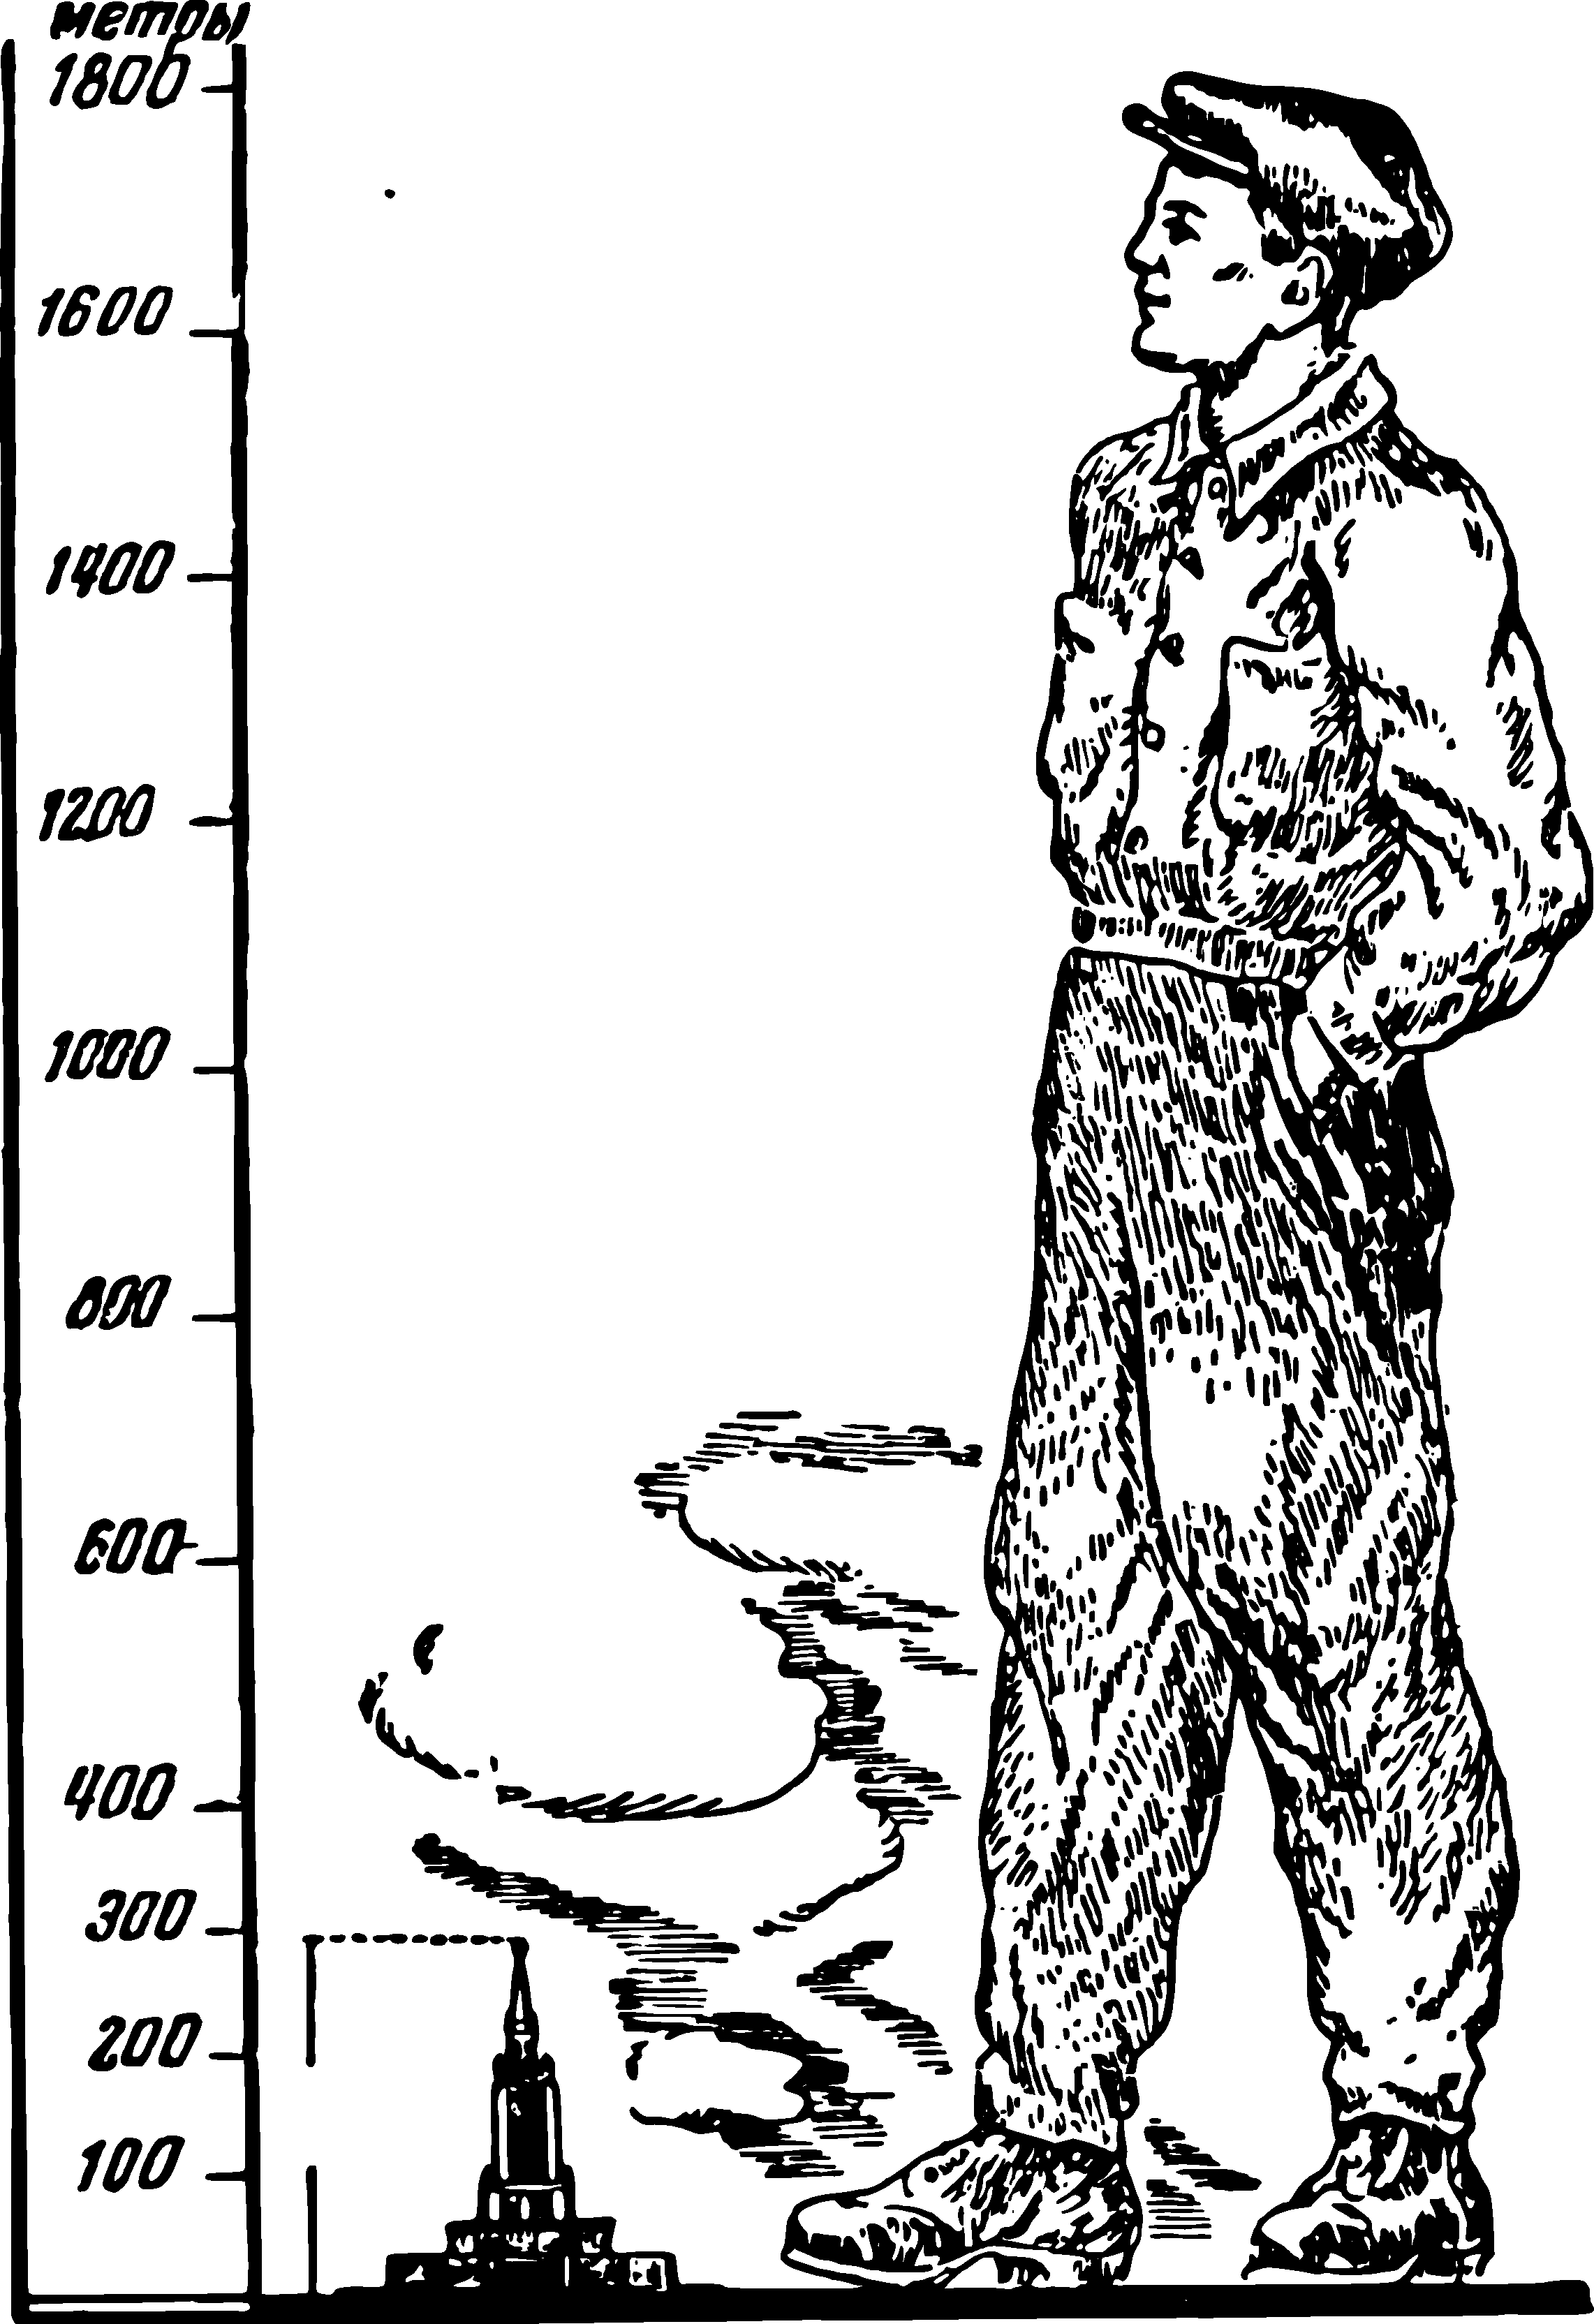
\includegraphics[width=0.6\textwidth]{figures/ch-11/fig-161.pdf}
\sidecaption{A young man magnified 1000 times.\label{fig-161}}
\end{figure}




\begin{center}
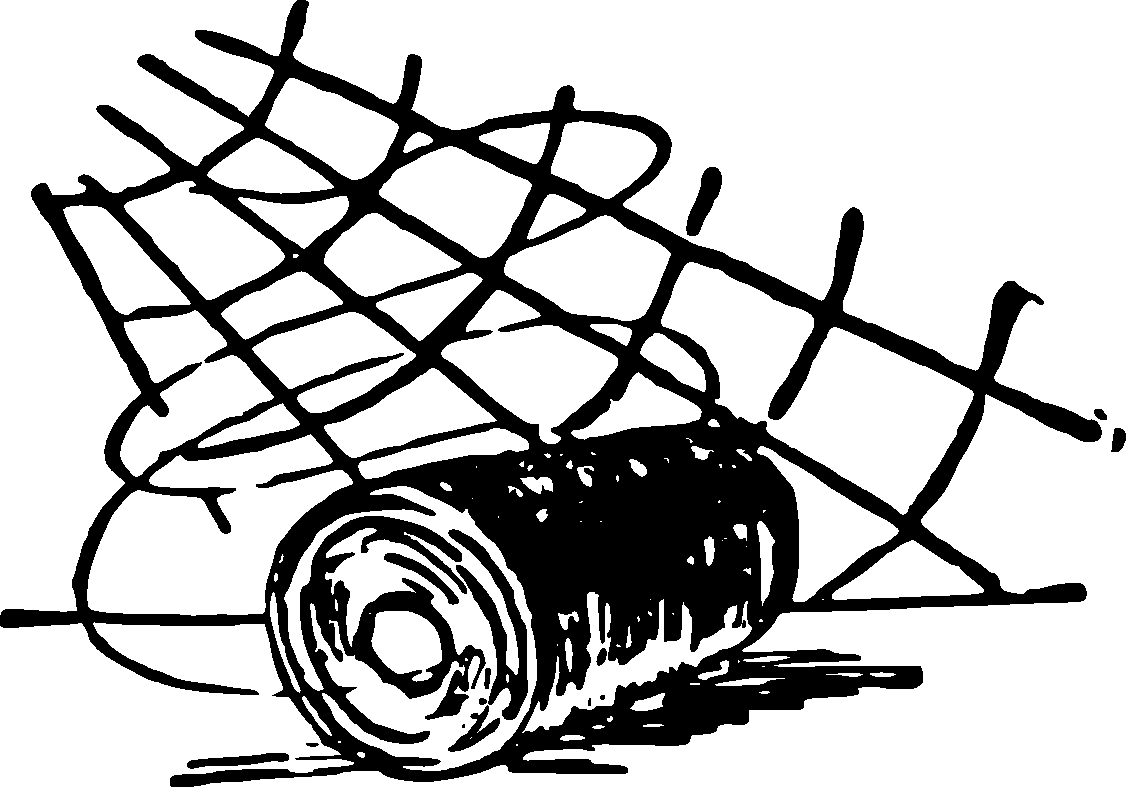
\includegraphics[width=0.3\textwidth]{figures/ch-11/fig-ch-11-tail.pdf}
\end{center}


















